
\begin{frame}{(Kan) Composition Structure}
	\centering
	\uncover<2->{We need our types to have a \textbf{composition structure}}.

	\uncover<3->{Lots of different variations!}

	\uncover<4->{Agda uses \textbf{homogeneous composition} and \textbf{transport}.}
\end{frame}

\begin{frame}{Cubical Subtypes}
	\centering
	Let $u : A$ be a \alert{partial element} in a \alert{restricted context} $\Gamma, \phi$.

	\uncover<2->{$A[\varphi \mapsto u]$ is the \textbf{cubical subtype} of elements $x : A$ such that $\varphi \implies x \equiv u$.}
\end{frame}

% CHM (1802.01170) pg 11 - we borrow notation from there, but use A instead of D(u) and the proper
% notation for substitution (like the one we saw in semantics)
\begin{frame}{Homogeneous Composition}
	\centering
	\begin{equation*}
	\inferrule*
	{
		\Gamma \entails \only<2>{\hlmathy{color_mbgreen}}{A \mathrel{\mathsf{type}}}
		\and
		\Gamma \entails \only<3>{\hlmathy{color_mbgreen}}{\varphi : \mathbb{F}}
		\and
		\Gamma, j : \mathbb{I}, \varphi \entails \only<4,8>{\hlmathy{color_mbgreen}}{u : A}
		\and
		\Gamma \entails \only<5,8>{\hlmathy{color_mbgreen}}{u_0 : A [\varphi \mapsto u[0/j]]}
	}
	{
		\uncover<6->{\Gamma \entails \alert{\mathsf{hcomp}}^j_A\,[\varphi \mapsto u] u_0 \defcolon A[\only<7>{\hlmathy{color_msgreen}}{\varphi \mapsto u[1 / j]}]}
	}
	\end{equation*}

	\uncover<8->{If $u$ and $u_0$ form an \textbf{open box}, then $\mathsf{hcomp}$ lets us \textbf{close} the box (by giving us $u_1$).}
\end{frame}

\begin{frame}[t]{Example | Transitivity}
	\begin{center}
		Let's prove \textbf{transitivity}.
	\end{center}
	\vskip\bigskipamount
	\begin{columns}
		\begin{column}{0.6\textwidth}
			\centering
			\uncover<2->{
			Suppose $x, y, z : A$.
			\vskip\medskipamount
			\cleanalign{\centering}{\begin{aligned}
				- \pathcom - &\defcolon (x = y) \to (y = z) \to (x = z) \phantom{\ (p i)}\\
				\vphantom{[\begin{smallmatrix*}[l]{(i = 0) \mapsto x}\\{(i = 1) \mapsto q\,j}\end{smallmatrix*}]} % To prevent line moving slightly up/down.
				\only<2>{{-} \pathcom {-} &\equiv {?}}
				\only<3>{{-} \pathcom {-} &\equiv \lambda p.\ \lambda q.\ {?}}
				\only<4-11>{{-} \pathcom {-} &\equiv \lambda p.\ \lambda q.\ \lambda i.\ {?}}
				\only<12>{{-} \pathcom {-} &\equiv \lambda p.\ \lambda q.\ \lambda i.\ \mathsf{hcomp}^j_A\,[\begin{smallmatrix*}[l]{(i = 0) \mapsto x}\\{(i = 1) \mapsto q\,j}\end{smallmatrix*}] (p\,i)}
			\end{aligned}}
			}
			\vskip\medskipamount
			\uncover<2-11>{
			\begin{boxybox}
				\begin{flushleft}
					\cleanalign{\centering}{\begin{aligned}
						\only<2>{\textsc{Goal: }& (x = y) \to (y = z) \to (x = z)}
						\only<3>{\textsc{Goal: }& x = z}
						\only<4->{\textsc{Goal: }& A}
					\end{aligned}}
				\end{flushleft}
			\end{boxybox}
			}
			\uncover<4-11>{
			\begin{boxybox}
				\begin{flushleft}
					\cleanalign{\centering}{\begin{aligned}
						\textsc{Boundary: }& (i = 0) \mapsto x\\
						&(i = 1) \mapsto z
					\end{aligned}}
				\end{flushleft}
			\end{boxybox}
			}
		\end{column}
		% Hint - use \fbox{...} to box around a column if you want to kinda-preview it's border.
		\begin{column}{0.4\textwidth}
			\centering
			\begin{tikzpicture}[scale=1,black,x=1pt,y=1pt,every node/.style={scale=0.6}]
				\useasboundingbox (-48, -48) rectangle (96, 96);
				% Points
				\coordinate (TL) at (0, 48);
				\coordinate (TR) at (48, 48);
				\coordinate (BR) at (48, 0);
				\coordinate (BL) at (0, 0);
		
				\coordinate (ZI) at ($(TL) + (0, 32)$);
				\coordinate (UI) at ($(TR) + (0, 32)$);
				\coordinate (ZJ) at ($(TL) + (-32, 0)$);
				\coordinate (UJ) at ($(BL) + (-32, 0)$);
				\coordinate (ZIR) at ($(BL) + (0, -32)$);
				\coordinate (UIR) at ($(BR) + (0, -32)$);
				\coordinate (ZJR) at ($(TR) + (32, 0)$);
				\coordinate (UJR) at ($(BR) + (32, 0)$);
		
				
				% Interval
				\only<4->{
				\draw (ZI) -- (UI);
				\draw ($(ZI)+(0,-2)$) -- ($(ZI)+(0,2)$) node[above] {$0$};
				\draw ($(UI)+(0,-2)$) -- ($(UI)+(0,2)$) node[above] {$1$};
				\draw ($(ZI)!0.5!(UI) + (0,2)$) node[above] {$i$}
				;
				}

				\only<5->{
				\draw (ZJ) -- (UJ);
				\draw ($(ZJ)+(2, 0)$) -- ($(ZJ)+(-2, 0)$) node[left] {$0$};
				\draw ($(UJ)+(2,0)$) -- ($(UJ)+(-2, 0)$) node[left] {$1$};
				\draw ($(ZJ)!0.5!(UJ) + (-2, 0)$) node[left] {$j$};
				}
				
				\only<7->{
					% Dashed projections
					\draw[dashed]
					(ZI) -- (TL)
					(UI) -- (TR)
					;
				}
				\only<10->{
					\draw[dashed] (ZJ) -- (TL);
				}
				\only<11->{
					\draw[dashed] (UJ) -- (BL);
				}

				\only<6->{
				% Square background
				\draw[line width=0,fill=color_fill_default]
				(TL) --
				(TR) --
				(BR) --
				(BL) --
				cycle;
				% Grays
				\draw[line width=1.5pt, color_shaded_default]
					(TL) -- (TR) -- (BR) -- (BL) -- cycle
					;
				}
				
				\only<7->{
					\fill[color_flame]
						(ZI) circle(2pt)
						(UI) circle(2pt)
						;
				}

				\only<8->{
					\draw ($(TL)!0.5!(BL)$) node[left=4pt] {$x$};
					\draw[line width=1.5pt, magenta]
						(TL) -- (BL);
					\fill[magenta]
						(TL) circle(2pt) node[above left] {$x$}
						(BL) circle(2pt) node[below left] {$x$}
						;
				}
				
				\only<9->{
					\draw ($(TR)!0.5!(BR)$) node[right=4pt] {$q\, j$};
					\draw[line width=1.5pt, magenta]
						(TR) -- (BR);
					\fill[magenta]
						(TR) circle(2pt) node[above right] {$y$}
						(BR) circle(2pt) node[below right] {$z$}
						;
				}

				\only<10->{
					\draw ($(TL)!0.5!(TR)$) node[above=4pt] {$p\,i$};
					\draw[line width=1.5pt, color_blue]
						(TL) -- (TR);
					\fill[color_electric_purple]
						(TL) circle(2pt) node[above left] {$x$}
						(TR) circle(2pt) node[above right] {$y$}
						;
					\fill[color_cerulean_crayola]
						(ZJ) circle(2pt)
						;
				}
				\only<11->{
					\draw ($(BL)!0.5!(BR)$) node[below=4pt] {$\mathsf{hcomp}$};
					\draw[line width=1.5pt, color_blue]
						(BL) -- (BR);
					\fill[color_electric_purple]
						(BL) circle(2pt) node[below left] {$x$}
						(BR) circle(2pt) node[below right] {$z$}
						;
					\fill[color_cerulean_crayola]
						(UJ) circle(2pt)
						;
				}
				% 
		
				% Highlights

				%\draw[line width=1.5pt, color_blue]
				%	(BL) -- (BR);
				%\fill[color_blue]
				%	(BR) circle(2pt)
				%	;

				%\fill[color_electric_purple] (BL) circle(2pt);
				
			\end{tikzpicture}
		\end{column}
	\end{columns}
\end{frame}

\begin{frame}{Generalized Transport}
	\centering
	\begin{equation*}
	\inferrule*
	{
		\Gamma, i : \mathbb{I} \entails \only<2>{\hlmathy{color_mbgreen}}{A \mathrel{\mathsf{type}}}
		\and
		\Gamma \entails \only<3>{\hlmathy{color_mbgreen}}{\varphi : \mathbb{F}}
		\and
		\Gamma, i : \mathbb{I}, \varphi \entails \only<4>{\hlmathy{color_mbgreen}}{A \equiv A[0/i]}
		\and
		\Gamma \entails \only<5>{\hlmathy{color_mbgreen}}{u_0 : A [0/i]}
	}
	{
		\uncover<6->{\Gamma \entails \alert{\mathsf{transp}}^i\, A\, \varphi\, u_0 \defcolon A[\only<7>{\hlmathy{color_msgreen}}{1/i}][\only<8>{\hlmathy{color_msgreen}}{\varphi \mapsto u_0}]}
	}
	\end{equation*}
\end{frame}

\begin{frame}{Example | Transport}
	\centering
	We can now \textbf{transport} a point along an \alert{equality} of types.
	\begin{align*}
		\mathsf{transport}_{A, B} &\defcolon A \equiv B \to A \to B\\
		\mathsf{transport}_{A, B} &\equiv \lambda p.\, \lambda x.\,\mathsf{transp}^i\,  (p\, i)\, \only<2>{\hlmathy{color_msgreen}}{0_\mathbb{F}}\, x
	\end{align*}
	\uncover<3->{
	Transport along a \alert{constant} path \textbf{reduces} to the input:
	\begin{align*}
		\mathsf{transportRefl} &\defcolon \only<4>{\hlmathy{color_msgreen}}{\mathsf{transport}_{A, A}\, (\mathsf{refl}\, A)\, x} = \only<5>{\hlmathy{color_msgreen}}{x}\\
		\mathsf{transportRefl} &\equiv \lambda i.\, \mathsf{transp}^i\, A\, \only<4-5>{\hlmathy{color_msgreen}}{(i = 1)}\, x
	\end{align*}
	}
\end{frame}

\begin{frame}{Higher Inductive Types}
	\centering
	Constructors of \textbf{higher inductive types} can produce points, paths, paths between paths \dots
\end{frame}

\begin{frame}{What's Not Covered Here?}
	\begin{itemize}
		\uncover<2->{\item \textbf{Glue}/\textbf{equivalence extension} types: used to prove \textbf{univalence}:}
		\begin{itemize}
			\uncover<3->{\item $(A \simeq B) \simeq (A = B)$}
			\uncover<4->{\item Nice consequences for mathematics (e.g. \alert{univalent} categories).}
		\end{itemize}
		\uncover<5->{\item \textbf{Dependent} path types: dependent functions out of the interval.}
		\begin{itemize}
			\uncover<6->{\item We can define these using $\mathsf{trans}$.}
			\uncover<7->{\item Agda defines path types \textit{in terms} of dependent path types.}
		\end{itemize}
		\uncover<8->{\item \textbf{Swan} identity types, which support \emph{judgemental} path induction.}
	\end{itemize}
\end{frame}

\begin{frame}{What's Next?}
	\begin{itemize}
		\uncover<2->{\item \textbf{Cartesian} cubical type theory: no ${\land}, {\lor}, {\neg}$, but has $(r = s)$.}
			\begin{itemize}
				\uncover<3->{\item Implemented in the experimental \textcolor{color_blue}{cooltt}.}
			\end{itemize}
			\uncover<4->{\item \textbf{Extension types}: generalized path types for user-provided cofibrations.}
			\uncover<5->{\item Other cube categories being investigated: \textbf{Dedekind}, \textbf{disjunctive}, \textbf{semicartesian}\dots}
			\uncover<6->{\item \textbf{XTT}, a non-univalent cubical type theory with \textbf{regularity} and \textbf{UIP}.}
			\uncover<7->{\item \textbf{HOTT}, a (\alert{work-in-progress}) univalent type theory with \textbf{observational} identity types.}
		\begin{itemize}
			\uncover<8->{\item $\mathsf{Id}_{A \times B}(\dots) \equiv \mathsf{Id}_A(\dots) \times \mathsf{Id}_B(\dots)$}
		\end{itemize}
	\end{itemize}
\end{frame}

\begin{frame}[plain,t]{Cubical Resources | agda/cubical}
	\centering
	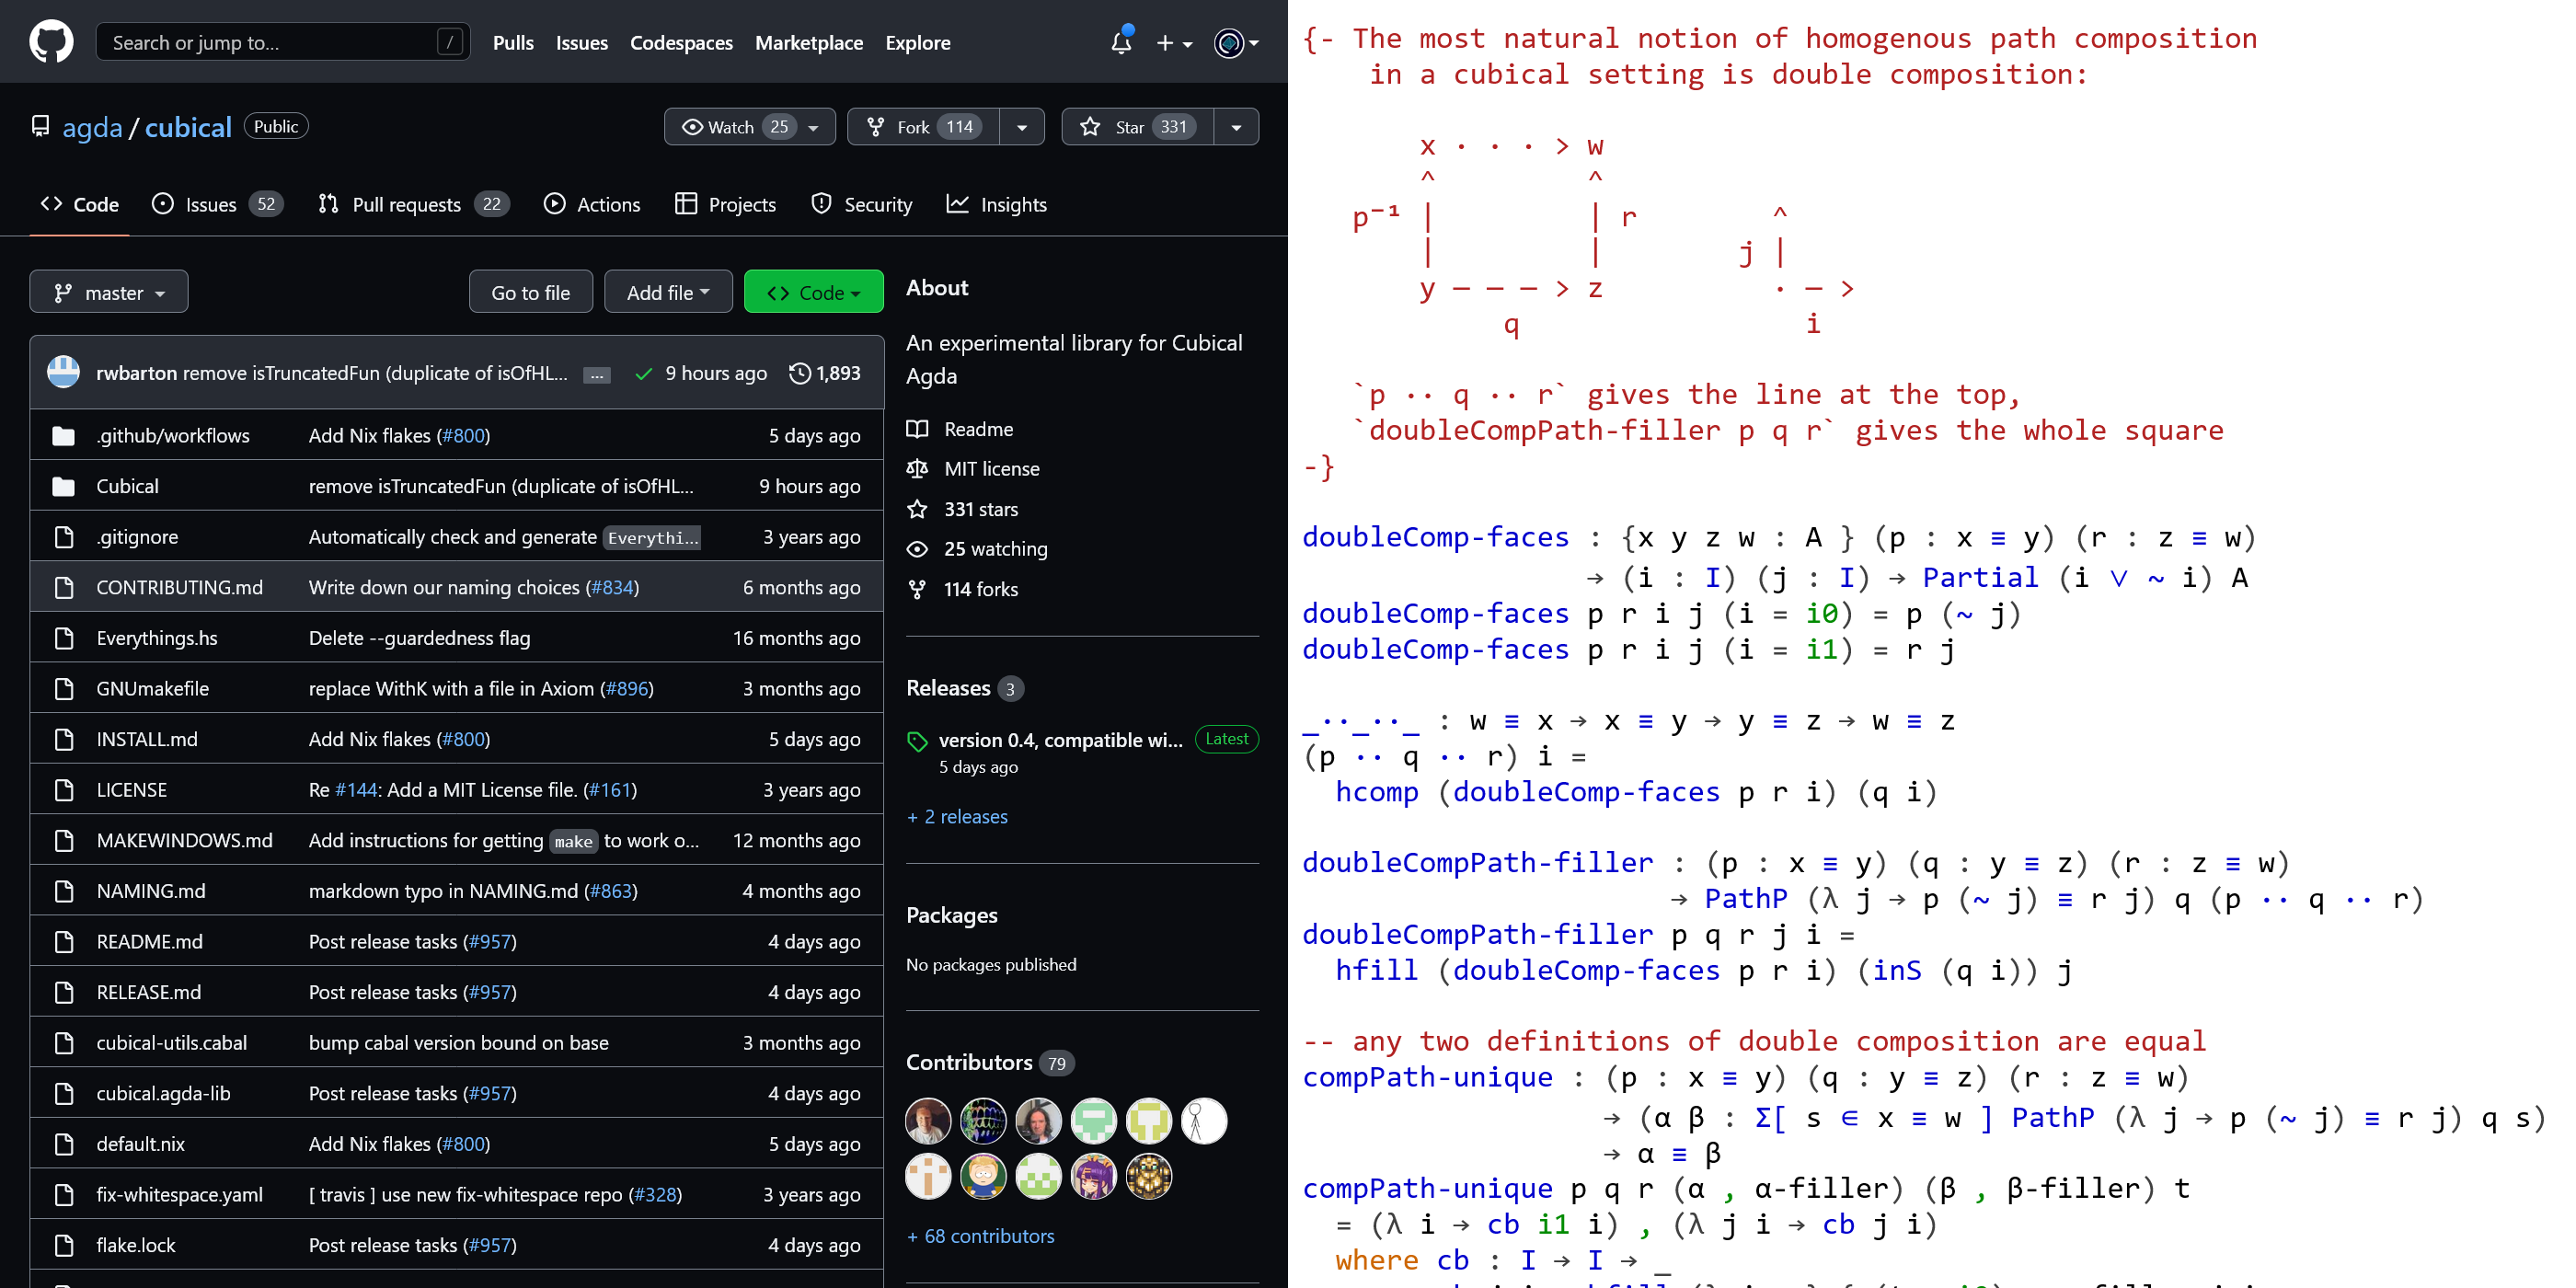
\includegraphics[width=0.9\textwidth]{../res/agda-cubical.png}

	github.com/agda/cubical

\end{frame}

\begin{frame}[plain,t]{Cubical Resources | The 1lab}
	\centering
	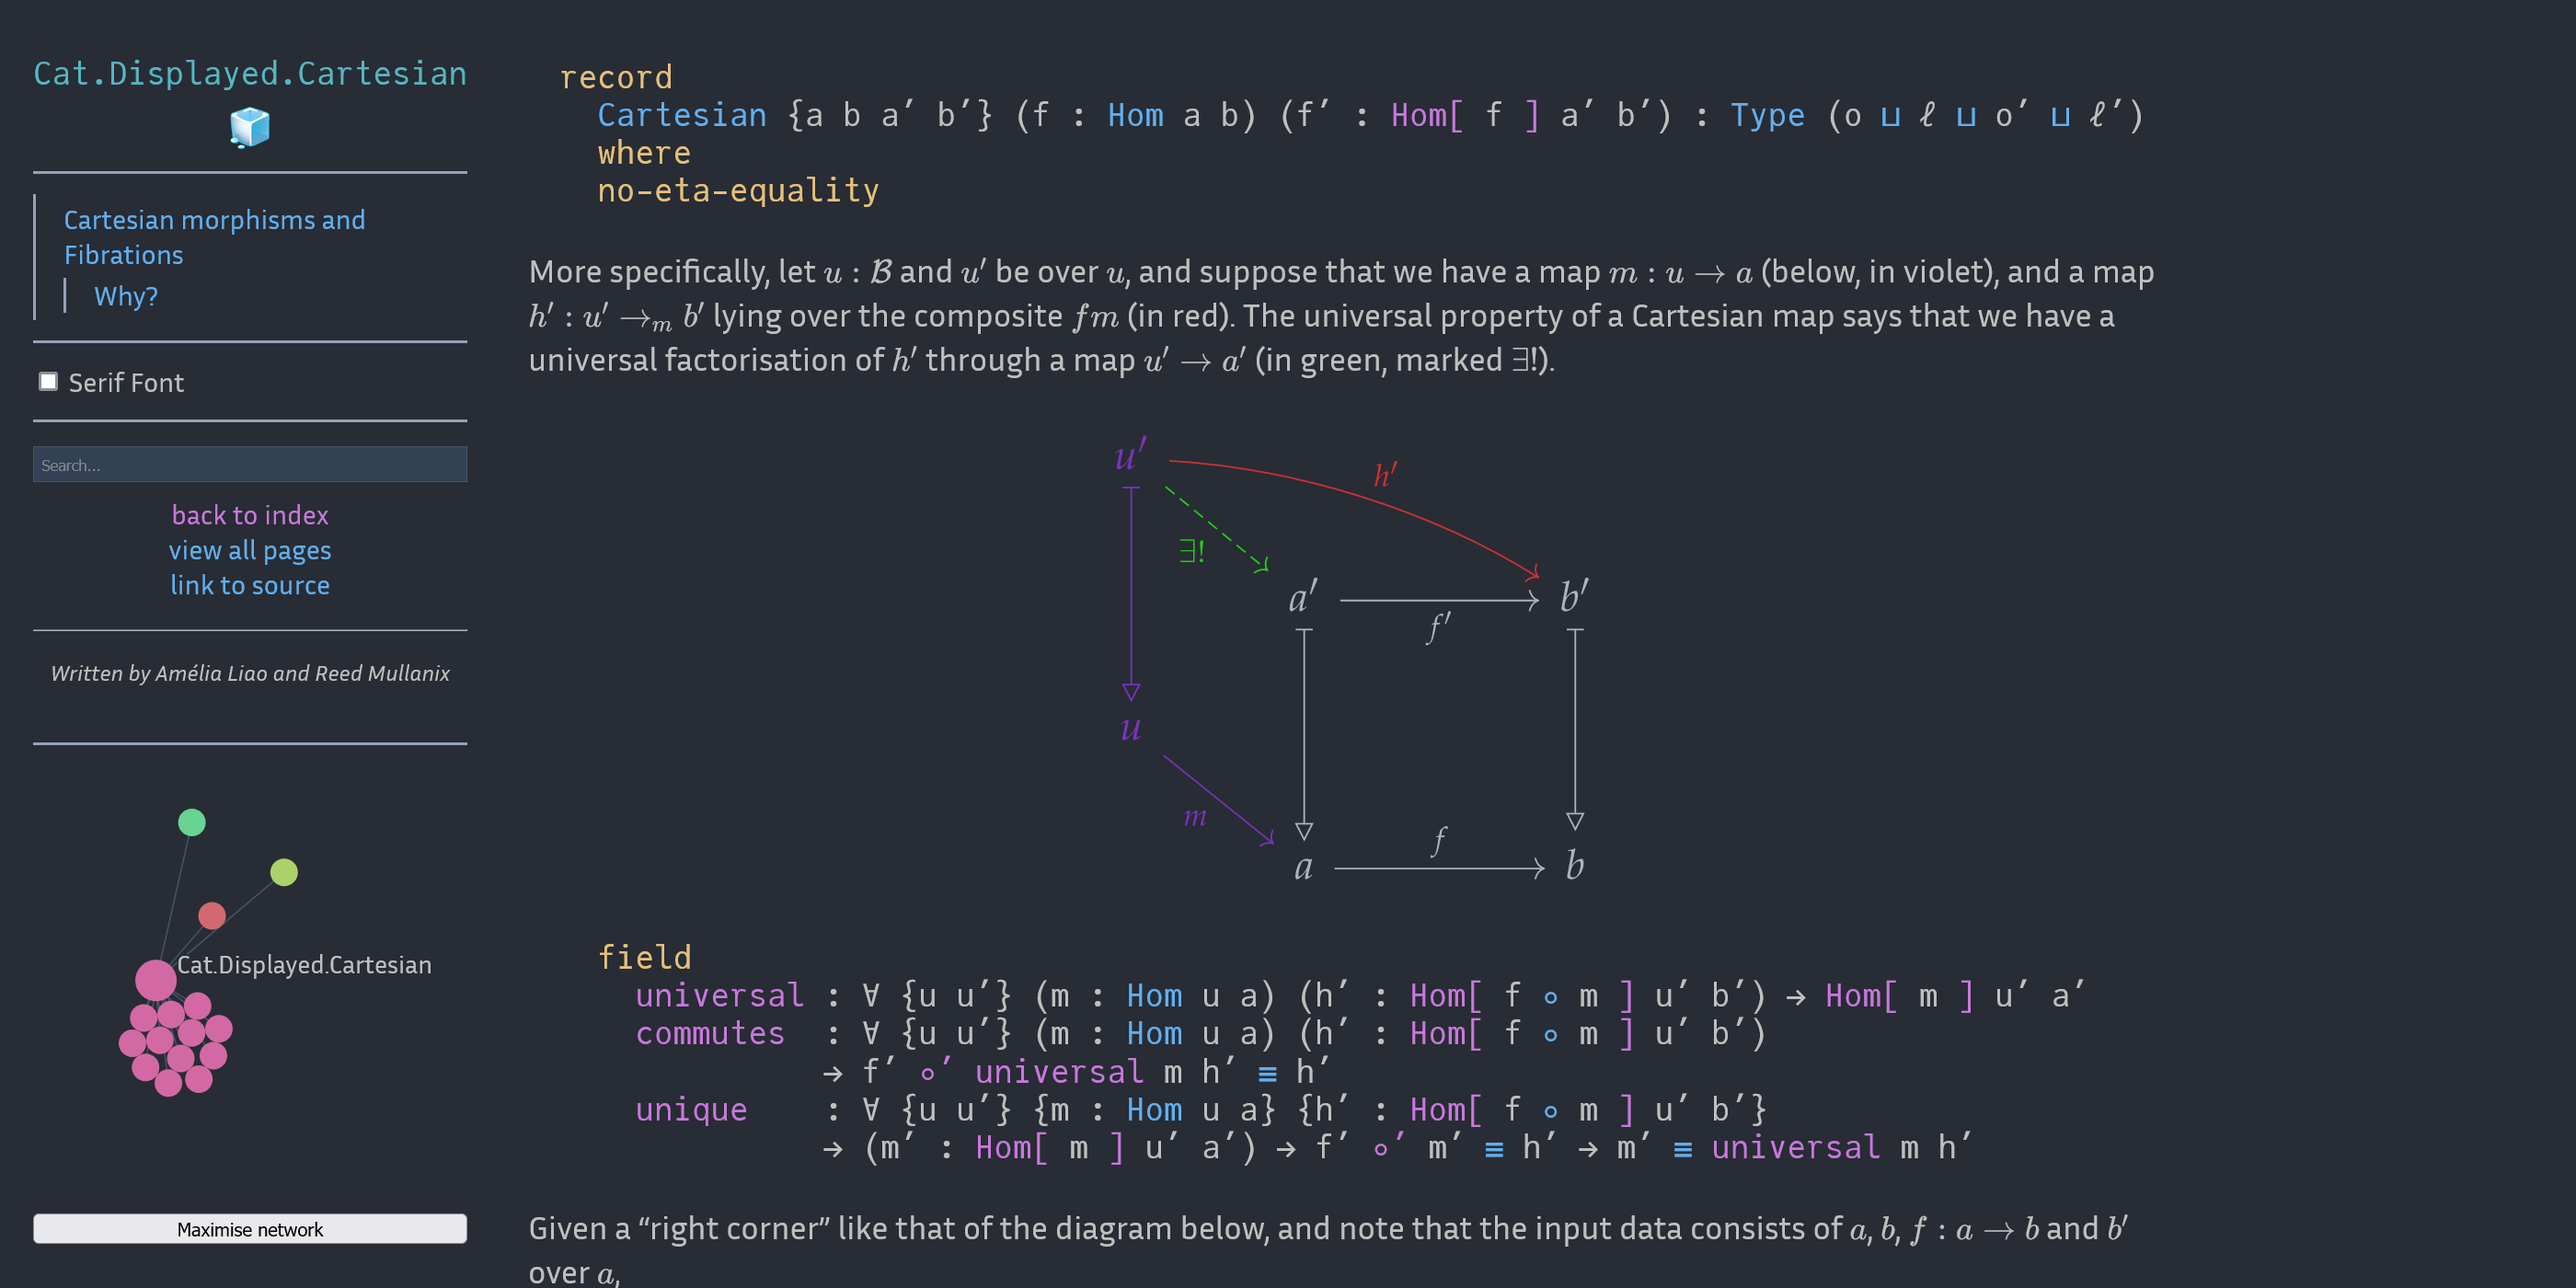
\includegraphics[width=0.9\textwidth]{../res/1lab-cartesian.png}

	1lab.dev
\end{frame}

\begin{frame}[plain]
	\centering
	Thank you!
\end{frame}